\documentclass[12pt, a4paper]{article}

% =============================================
% 1. Standard Packages for pdflatex
% =============================================
% The original file was configured for XeLaTeX with specific fonts ('TH Sarabun New', 'Cambria Math')
% that are likely not installed on your system, causing compilation to fail.
% The configuration has been changed to use the standard 'pdflatex' compiler,
% which is more common and doesn't require special fonts.
\usepackage[utf8]{inputenc}
\usepackage[T1]{fontenc}

% =============================================
% 2. แพ็กเกจ (Packages)
% =============================================
\usepackage{tikz}
\usetikzlibrary{shapes,arrows,positioning,fit,backgrounds}
\usepackage{geometry}
\geometry{top=2.5cm, bottom=2.5cm, left=2.54cm, right=2.54cm}
\usepackage{graphicx}
\usepackage{float}
\usepackage{multirow}
\usepackage{hyperref}
\usepackage{indentfirst}
\usepackage{placeins} % Added to control float placement
\usepackage{setspace}
\usepackage{amsmath}
\raggedbottom
\setlength{\parskip}{0pt}
\setlength{\parsep}{0pt}

% =============================================
% 3. หัวข้อ (Headers Format)
% =============================================
\usepackage{titlesec}
\newcommand{\sectionbreak}{\clearpage}
\titleformat{\section}
  {\centering\bfseries\fontsize{20}{24}\selectfont}{\thesection.}{0.4em}{}
\titleformat{\subsection}
  {\bfseries\fontsize{16}{20}\selectfont}{\thesubsection}{0.4em}{}
\titleformat{\subsubsection}
  {\bfseries\fontsize{14}{18}\selectfont}{\thesubsubsection}{0.4em}{}

% =============================================
% 4. เลขหน้า (Page Numbers)
% =============================================
\usepackage{fancyhdr}
\pagestyle{fancy}
\fancyhf{}
\renewcommand{\headrulewidth}{0pt}
\fancyfoot[R]{\thepage}

% =============================================
% 5. เริ่มเอกสาร (Begin Document)
% =============================================
\begin{document}
\thispagestyle{empty}
\setlength{\baselineskip}{17pt}

% ============================================================
% ปกหน้า (Title Page)
% ============================================================
\begin{center}
    % The following lines include university and department logos.
    % If you do not have the image files 'kmutt_logo.png' and 'fibo_logo.png'
    % in the 'report/' directory, compilation will fail. They are commented out for now.
    % \includegraphics[height=3.0cm]{kmutt_logo.png}
    % \hspace{0.5cm}
    % \includegraphics[height=3.0cm]{fibo_logo.png}
    \vspace{0.3cm}
    {\bfseries\fontsize{20}{24}\selectfont
    Development and Validation of a Hydraulic-Pressure \\
    Based Load Estimator for Static Wheel Loader}

    \vspace{0.8cm}
    {\fontsize{16}{20}\selectfont
    By \\
    Phattanarat Jeedjeen \\
    Institute of Field Robotics (FIBO) \\
    King Mongkut's University of Technology Thonburi \\
    \vspace{0.3cm}
    August 7, 2026
    }
\end{center}

\vspace{0.5cm}
\tableofcontents
\clearpage

\fontsize{14}{17}\selectfont
\setlength{\baselineskip}{17pt}

% ==================================================================
% Section 1: Introduction
% ==================================================================
\section{Introduction}

\subsection{Background}
In modern industrial facilities, autonomous wheel loaders are critical for managing bulk biomass, such as scooping wood piles for furnace feeding and pile organization. However, a major gap exists in their ability to physically perceive and quantify payloads during the excavation phase. Operating ``blindly'' without human senses, these loaders struggle with the variable density of wood piles, often resulting in empty or under-loaded buckets that lead to wasted fuel, unnecessary machine wear, and operational bottlenecks. 

To resolve this, developing a Hydraulic-Pressure Based Load Estimator utilizing sensors on the lift cylinder will allow the system to calculate payload weight within a few seconds. This enables crucial payload verification, acting as a quality-control checkpoint that aborts transport and triggers a re-scoop if the load falls below a specific threshold, thereby eliminating inefficient ``dry runs''. Furthermore, knowing the precise weight allows the control system to implement adaptive kinematic control, dynamically adjusting velocity and acceleration profiles to account for changes in the machine's center of gravity and momentum. Transforming the loader into an intelligent, physically-aware system.

\subsection{Scope and Operational Constraints}
To ensure accurate payload verification and simplify the initial physical models, the development and validation of the load estimation system will be bound by the following scope and assumptions:
\begin{enumerate}
    \item \textbf{Target Machinery}: The algorithms, physical dimensions, and sensor calibrations will be exclusively developed for the XCMG958 wheel loader.
    \item \textbf{Static Conditions}: Rather than performing dynamic load weighing on the move, the mass estimation will be executed entirely under static conditions. The system will only record and process pressure sensor data after the boom has been lowered and the machine has come to a complete stop.
    \item \textbf{Environmental and Posture Requirements}: To eliminate the effects of gravity offsets and external momentum, the loader must be stationary on flat, level ground during the measurement. Furthermore, the implement must be curled into a maximum tilt bucket posture to standardize the mechanical leverage.
    \item \textbf{Center of Gravity Assumption}: For the physical model calculations, the payload is assumed to be distributed symmetrically, with the resultant center of gravity acting directly downward through the geometric center of the bucket.
    \item \textbf{Boom Angular Range}: The system will only validate and process load estimations when the boom angle—tracked by the encoder at the boom-chassis pin—falls within a carefully specified operating range. Readings outside this angular window will be discarded to prevent kinematic calculation errors.
\end{enumerate}

\subsection{Objectives}
The primary goal of this project is to develop and validate a hydraulic-pressure based load estimator specifically for the XCMG958 autonomous wheel loader. To achieve this, the project targets the following specific objectives:
\begin{enumerate}
    \item \textbf{Preventing ``Run Dry'' Operations}: To establish a quality-control checkpoint immediately following the scooping phase. By verifying the payload, the system can abort transport and command a re-scoop if the load falls below a predefined weight threshold, thereby eliminating unnecessary empty transport cycles.
    \item \textbf{High-Speed Estimation}: To ensure the real-time mass calculation is highly efficient, with the entire estimation process completed within a strict maximum timeframe of 3 seconds.
    \item \textbf{Target Accuracy and Sensor Fusion}: To accurately calculate payload weight by fusing data from a pressure sensor installed on the lift cylinder with positional data from a rotary encoder at the boom-chassis pin. This integrated system must achieve an estimation accuracy of within $\pm 5\%$ of the machine's full load capacity (3.2 tons).
\end{enumerate}

% ==================================================================
% Section 2: Modeling and Algorithm Development
% ==================================================================
\section{Modeling and Algorithm Development}
The final load estimation is the result of a multi-stage process that filters raw sensor data, models physical behavior, and applies data-driven compensations to correct for model inaccuracies.

\subsection{Simple Beam Model}
\begin{figure}[H]
    \centering
    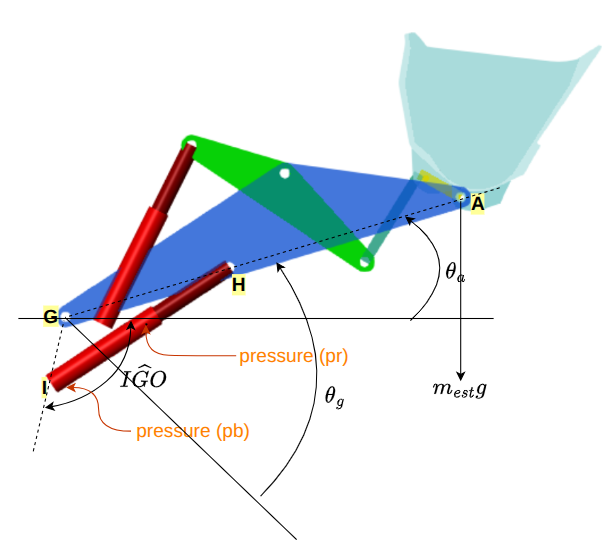
\includegraphics[width=0.7\textwidth]{../simple_beam.png}
    \caption{Simple Beam Model representing the loader's arm-bucket assembly}
\end{figure}

To translate the force from the hydraulic cylinders into an estimated load, the arm-bucket assembly is modeled as a \textbf{simple beam system}. This provides a physics-based initial estimate of the bucket load ($w_{simple}$) based on the known geometry and the calculated cylinder force.

\begin{enumerate}
    \item \textbf{Cylinder Force ($F_c$)}:
    \begin{equation}
        F_c = 2 \cdot (A_b \cdot (p_b - p_{b\_offset}) - A_r \cdot (p_r - p_{r\_offset})) \cdot C
    \end{equation}
    
    \item \textbf{Geometry Factor ($a$)}:
    \begin{equation}
        a = \sin(HIO) - \cos(HIO) \cdot \tan(\theta_a)
    \end{equation}
    where $HIO$, $GIH$, and $L_{ih}$ are intermediate geometric angles and lengths calculated from the loader's linkage constants and the current boom angle $\theta_a$.
    
    \item \textbf{Simple Load ($w_{simple}$)}:
    \begin{equation}
        w_{simple} = \left(\frac{F_c \cdot L_{gh}}{L_{ag}}\right) \cdot \frac{a}{g}
    \end{equation}
\end{enumerate}

\begin{table}[H]
    \centering
    \caption{Parameters for Simple Beam Model}
    \begin{tabular}{l|l|l}
        \hline
        \textbf{Parameter} & \textbf{Value} & \textbf{Description} \\
        \hline
        $A_b$ & $0.02 \text{ m}^2$ & Cross-sectional area of the cylinder bottom. \\
        $A_r$ & $0.014 \text{ m}^2$ & Cross-sectional area of the cylinder rod side. \\
        $C$ & $1220.7 \text{ Pa/ADC}$ & Conversion factor from sensor ADC to Pascals. \\
        $L_{gh}$ & $1.630 \text{ m}$ & Length of the main boom link. \\
        $L_{ag}$ & $3.9294 \text{ m}$ & Length of the lever arm from pivot to bucket. \\
        $L_{gi}$ & $0.654 \text{ m}$ & Length of the cylinder link. \\
        $IGO$ & $1.786 \text{ rad}$ & Fixed angle in the linkage geometry. \\
        $\theta_a$ & $\theta_g - 0.62 \text{ rad}$ & Processed boom angle, corrected with an offset. \\
        $g$ & $9.807 \text{ m/s}^2$ & Acceleration due to gravity. \\
        \hline
    \end{tabular}
\end{table}

\subsection{Load Estimation Algorithm}

\subsubsection{Signal Processing}
Raw data from the hydraulic pressure sensors and the boom angle encoder is inherently noisy. To ensure a stable and reliable input for the downstream calculations, \textbf{Exponential Moving Average (EMA)} filters are applied to both sensor streams. 

The filter is defined by the equation:
\begin{equation}
    y_t = \alpha \cdot x_t + (1 - \alpha) \cdot y_{t-1}
\end{equation}

\begin{table}[H]
    \centering
    \caption{Signal Processing Parameters}
    \begin{tabular}{l|l|l}
        \hline
        \textbf{Parameter} & \textbf{Value} & \textbf{Description} \\
        \hline
        $y_t$ & - & The filtered output at the current step. \\
        $x_t$ & - & The raw sensor input at the current step. \\
        $y_{t-1}$ & - & The filtered output from the previous step. \\
        $\alpha_{pressure}$ & $0.001$ & Smoothing factor for pressure sensors (low cutoff). \\
        $\alpha_{angle}$ & $0.1$ & Smoothing factor for the angle encoder (higher cutoff). \\
        \hline
    \end{tabular}
\end{table}

\subsubsection{Pressure Prediction}
To provide a rapid estimation without waiting for the hydraulic system to fully stabilize, a pressure estimator is used. This model treats the pressure response during a downward boom movement as a \textbf{first-order system}. By analyzing the initial transient pressure change $p(t)$ after the boom stops, the model can quickly predict the final pressure value $p_{final}$.

The final pressure is estimated using the formula:
\begin{equation}
    p_{final} = \frac{p(t) - p_{initial} \cdot e^{-t/\tau}}{1 - e^{-t/\tau}}
\end{equation}

\begin{table}[H]
    \centering
    \caption{Pressure Prediction Parameters}
    \begin{tabular}{l|l|l}
        \hline
        \textbf{Parameter} & \textbf{Value} & \textbf{Description} \\
        \hline
        $p_{final}$ & - & The predicted final pressure. \\
        $p(t)$ & - & The filtered pressure measured at time $t$. \\
        $p_{initial}$ & - & Initial pressure when the boom stops ($t=0$). \\
        $t$ & $0$ to $1.0 \text{ s}$ & Time elapsed since the boom became static. \\
        $\tau$ & $15.0 \text{ s}$ & Time constant of the first-order system ($0.25 \cdot T_s$). \\
        $T_s$ & $60.0 \text{ s}$ & Settling time of the hydraulic system. \\
        \hline
    \end{tabular}
\end{table}

\subsubsection{Regression Model}
\begin{quote}
\textit{Note: To get constant values ($c_1, c_2, c_3, k_1, k_2, k_3$), see the Calibration Procedure section. Constants must be adapted if a different wheel loader model is used.}
\end{quote}

\textbf{Empty Bucket Pressure Offset:}
The weight of the loader's arm and bucket assembly exerts force on the hydraulic cylinders, resulting in a baseline pressure reading even when empty. This offset varies with the boom angle $\theta_g$. 
\begin{equation}
    p_{b\_offset} = c_1 \cdot \theta_g + c_2
\end{equation}
\begin{equation}
    p_{r\_offset} = c_3
\end{equation}

\begin{table}[H]
    \centering
    \caption{Pressure Offset Model Parameters}
    \begin{tabular}{l|l|l}
        \hline
        \textbf{Parameter} & \textbf{Value} & \textbf{Description} \\
        \hline
        $c_1$ & $1699$ & Coefficient for the boom angle in $p_{b\_offset}$ model. \\
        $c_2$ & $4023$ & Intercept for the $p_{b\_offset}$ model (ADC value). \\
        $c_3$ & $413.3$ & Constant value for the $p_{r\_offset}$ model (ADC value). \\
        $\theta_g$ & - & The boom angle from the encoder (rad). \\
        \hline
    \end{tabular}
\end{table}

\textbf{Surface Fit Compensation:}
The simple beam model contains inaccuracies due to simplifying assumptions. A final compensation layer is applied via a linear model fitted to empirical datasets.
\begin{equation}
    load_{final} \text{ [ton]} = k_1 + k_2 \cdot w_{simple} \text{ [kg]} + k_3 \cdot \theta_g \text{ [rad]}
\end{equation}

\begin{table}[H]
    \centering
    \caption{Surface Fit Compensation Parameters}
    \begin{tabular}{l|l|l}
        \hline
        \textbf{Parameter} & \textbf{Value} & \textbf{Description} \\
        \hline
        $w_{simple}$ & - & Initial load estimate from Simple Beam Model (kg). \\
        $\theta_g$ & - & Raw boom angle from the encoder (rad). \\
        $k_1$ & $-0.2494$ & Intercept term (ton). \\
        $k_2$ & $1.0643 \times 10^{-3}$ & Coefficient for the simple model's output. \\
        $k_3$ & $0.51622$ & Coefficient for the boom angle. \\
        \hline
    \end{tabular}
\end{table}

% ==================================================================
% Section 3: Implementation
% ==================================================================
\section{Implementation}

\subsection{Software Architecture}
\begin{figure}[h!]
    \centering
    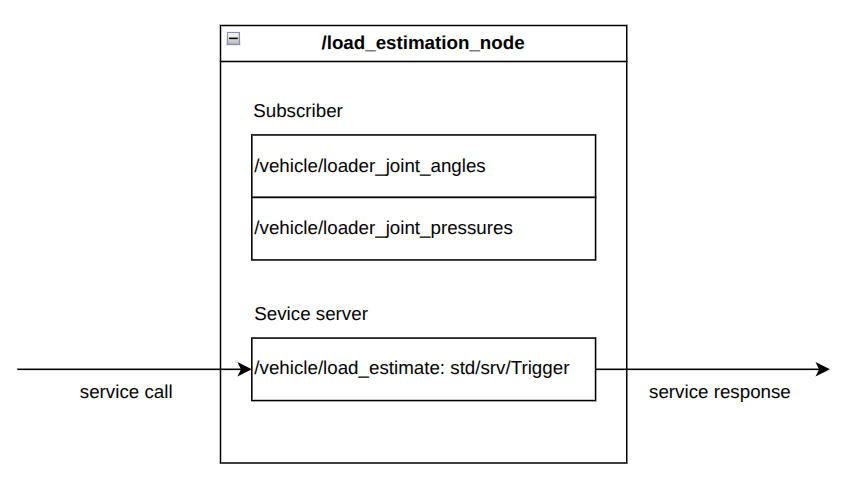
\includegraphics[width=0.8\textwidth]{../ros_structure.png}
    \caption{ROS 2 Structure for /load\_estimation\_node}
\end{figure}

The logic and multi-threaded architecture of the \texttt{load\_estimate.py} ROS 2 node are separated into three modular flows: Continuous Callbacks, Service Initialization, and Data Collection.

\subsubsection{Continuous Topic Callbacks (Angles \& Pressures)}
\begin{figure}[h!]
\centering
\resizebox{\textwidth}{!}{
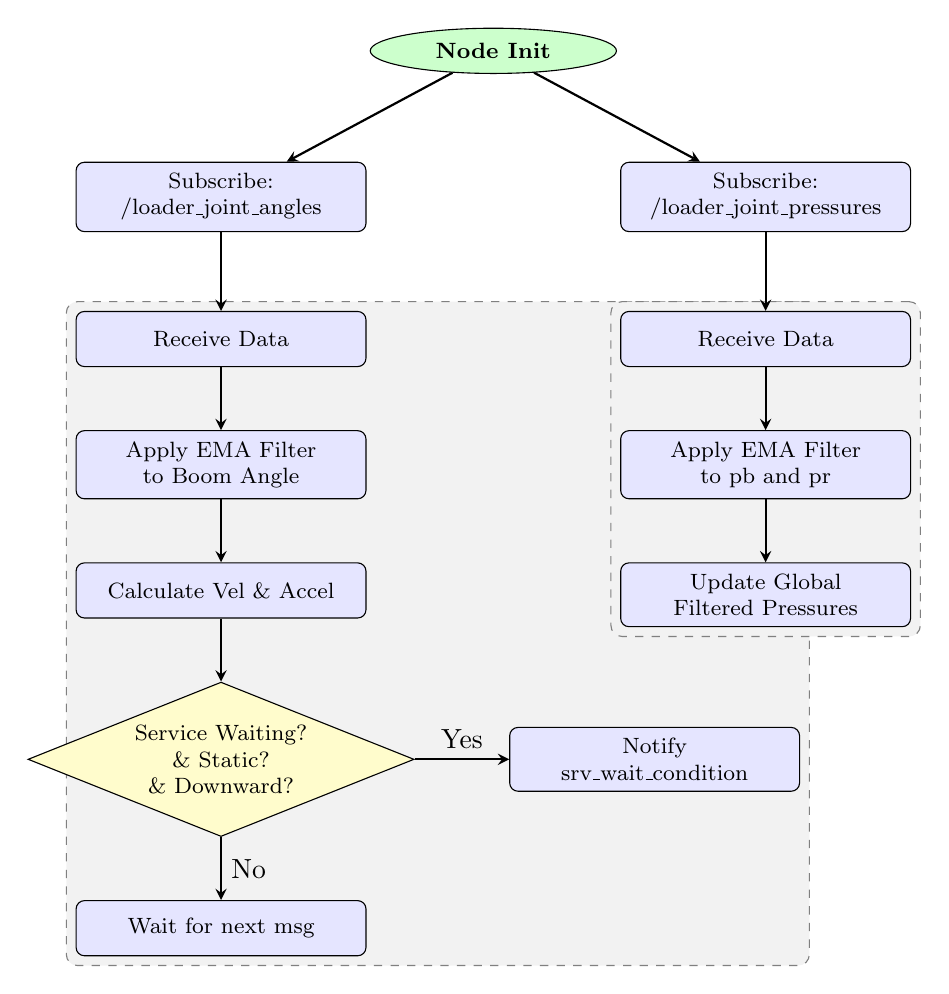
\begin{tikzpicture}[node distance=1.5cm, auto, >=latex']
    \tikzstyle{startend} = [draw, ellipse, fill=green!20, text width=2.0cm, text centered, font=\footnotesize\bfseries, inner sep=3pt]
    \tikzstyle{process}  = [draw, rectangle, fill=blue!10, text width=3.4cm, text centered, minimum height=0.7cm, rounded corners=3pt, font=\footnotesize, inner sep=4pt]
    \tikzstyle{decision} = [draw, diamond, fill=yellow!20, text width=2.2cm, text centered, aspect=2.5, font=\footnotesize, inner sep=1pt]
    \tikzstyle{arrow}    = [thick,->,>=stealth]

    % Main Start
    \node [startend] (init) {Node Init};

    % Subscribe blocks
    \node [process, below left=1.2cm and 0.5cm of init] (suba) {Subscribe:\\/loader\_joint\_angles};
    \node [process, below right=1.2cm and 0.5cm of init] (subp) {Subscribe:\\/loader\_joint\_pressures};

    % Angle Thread
    \node [process, below=1cm of suba] (a1) {Receive Data};
    \node [process, below=0.8cm of a1] (a2) {Apply EMA Filter\\to Boom Angle};
    \node [process, below=0.8cm of a2] (a3) {Calculate Vel \& Accel};
    \node [decision, below=0.8cm of a3, text width=2.5cm] (a4) {Service Waiting?\\\& Static?\\\& Downward?};
    \node [process, right=1.2cm of a4] (a5) {Notify\\srv\_wait\_condition};
    \node [process, below=0.8cm of a4] (a6) {Wait for next msg};

    % Pressure Thread
    \node [process, below=1cm of subp] (p1) {Receive Data};
    \node [process, below=0.8cm of p1] (p2) {Apply EMA Filter\\to pb and pr};
    \node [process, below=0.8cm of p2] (p3) {Update Global\\Filtered Pressures};

    % Connections
    \draw [arrow] (init) -- (suba);
    \draw [arrow] (init) -- (subp);
    
    \draw [arrow] (suba) -- (a1);
    \draw [arrow] (a1) -- (a2);
    \draw [arrow] (a2) -- (a3);
    \draw [arrow] (a3) -- (a4);
    \draw [arrow] (a4) -- node[above] {Yes} (a5);
    \draw [arrow] (a4) -- node[right] {No} (a6);

    \draw [arrow] (subp) -- (p1);
    \draw [arrow] (p1) -- (p2);
    \draw [arrow] (p2) -- (p3);
    
    % Grouping boxes
    \begin{pgfonlayer}{background}
        \node [fill=gray!10, rounded corners, draw=gray, dashed, fit=(a1) (a6) (a5)] {};
        \node [fill=gray!10, rounded corners, draw=gray, dashed, fit=(p1) (p3)] {};
    \end{pgfonlayer}
\end{tikzpicture}
}
\caption{Continuous Topic Callbacks (Angles \& Pressures Threading)}
\end{figure}
\FloatBarrier

\subsubsection{Service Call: Initialization \& Wait Conditions}
\begin{figure}[h!]
\centering
\resizebox{0.75\textwidth}{!}{
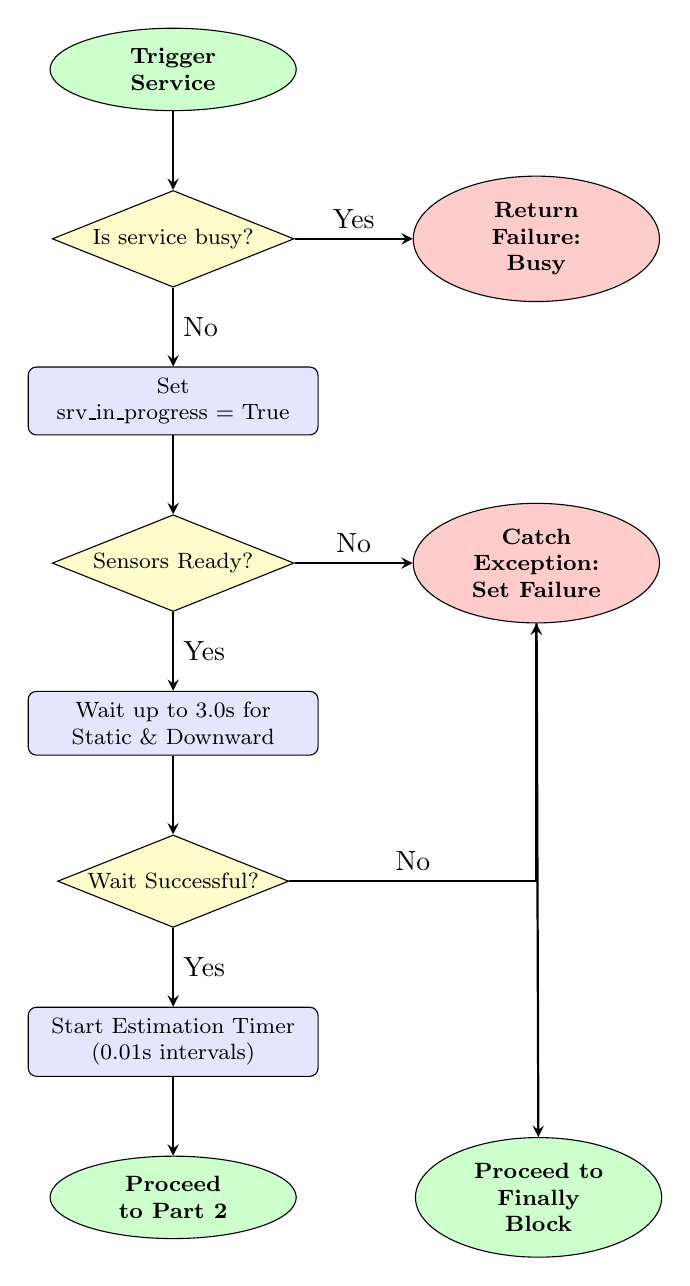
\begin{tikzpicture}[node distance=1.5cm, auto, >=latex']
    \tikzstyle{startend} = [draw, ellipse, fill=green!20, text width=2.0cm, text centered, font=\footnotesize\bfseries, inner sep=3pt]
    \tikzstyle{process}  = [draw, rectangle, fill=blue!10, text width=3.4cm, text centered, minimum height=0.7cm, rounded corners=3pt, font=\footnotesize, inner sep=4pt]
    \tikzstyle{decision} = [draw, diamond, fill=yellow!20, text width=2.2cm, text centered, aspect=2.5, font=\footnotesize, inner sep=1pt]
    \tikzstyle{success}  = [draw, ellipse, fill=red!20, text width=2.0cm, text centered, font=\footnotesize\bfseries, inner sep=3pt]
    \tikzstyle{arrow}    = [thick,->,>=stealth]

    \node [startend] (trig) {Trigger Service};
    \node [decision, below=1cm of trig] (busy) {Is service busy?};
    \node [success, right=1.5cm of busy] (fail1) {Return Failure:\\Busy};
    
    \node [process, below=1cm of busy] (settrue) {Set\\srv\_in\_progress = True};
    \node [decision, below=1cm of settrue] (ready) {Sensors Ready?};
    \node [success, right=1.5cm of ready] (catch) {Catch Exception:\\Set Failure};

    \node [process, below=1cm of ready] (wait) {Wait up to 3.0s for\\Static \& Downward};
    \node [decision, below=1cm of wait] (waitsuccess) {Wait Successful?};
    
    \node [process, below=1cm of waitsuccess] (starttimer) {Start Estimation Timer\\(0.01s intervals)};
    \node [startend, below=1cm of starttimer] (part2) {Proceed to Part 2};
    \node [startend, right=1.5cm of part2] (finally) {Proceed to\\Finally Block};

    \draw [arrow] (trig) -- (busy);
    \draw [arrow] (busy) -- node[above] {Yes} (fail1);
    \draw [arrow] (busy) -- node[right] {No} (settrue);
    
    \draw [arrow] (settrue) -- (ready);
    \draw [arrow] (ready) -- node[above] {No} (catch);
    \draw [arrow] (ready) -- node[right] {Yes} (wait);
    
    \draw [arrow] (wait) -- (waitsuccess);
    \draw [arrow] (waitsuccess) -| node[above, pos=0.25] {No} (catch);
    \draw [arrow] (waitsuccess) -- node[right] {Yes} (starttimer);
    
    \draw [arrow] (starttimer) -- (part2);
    \draw [arrow] (catch) -- (finally);
\end{tikzpicture}
}
\caption{Service Call: Initialization \& Wait Conditions}
\end{figure}
\FloatBarrier

\subsubsection{Service Call: Data Collection \& Final Calculation}
\begin{figure}[h!]
\centering
\resizebox{0.75\textwidth}{!}{
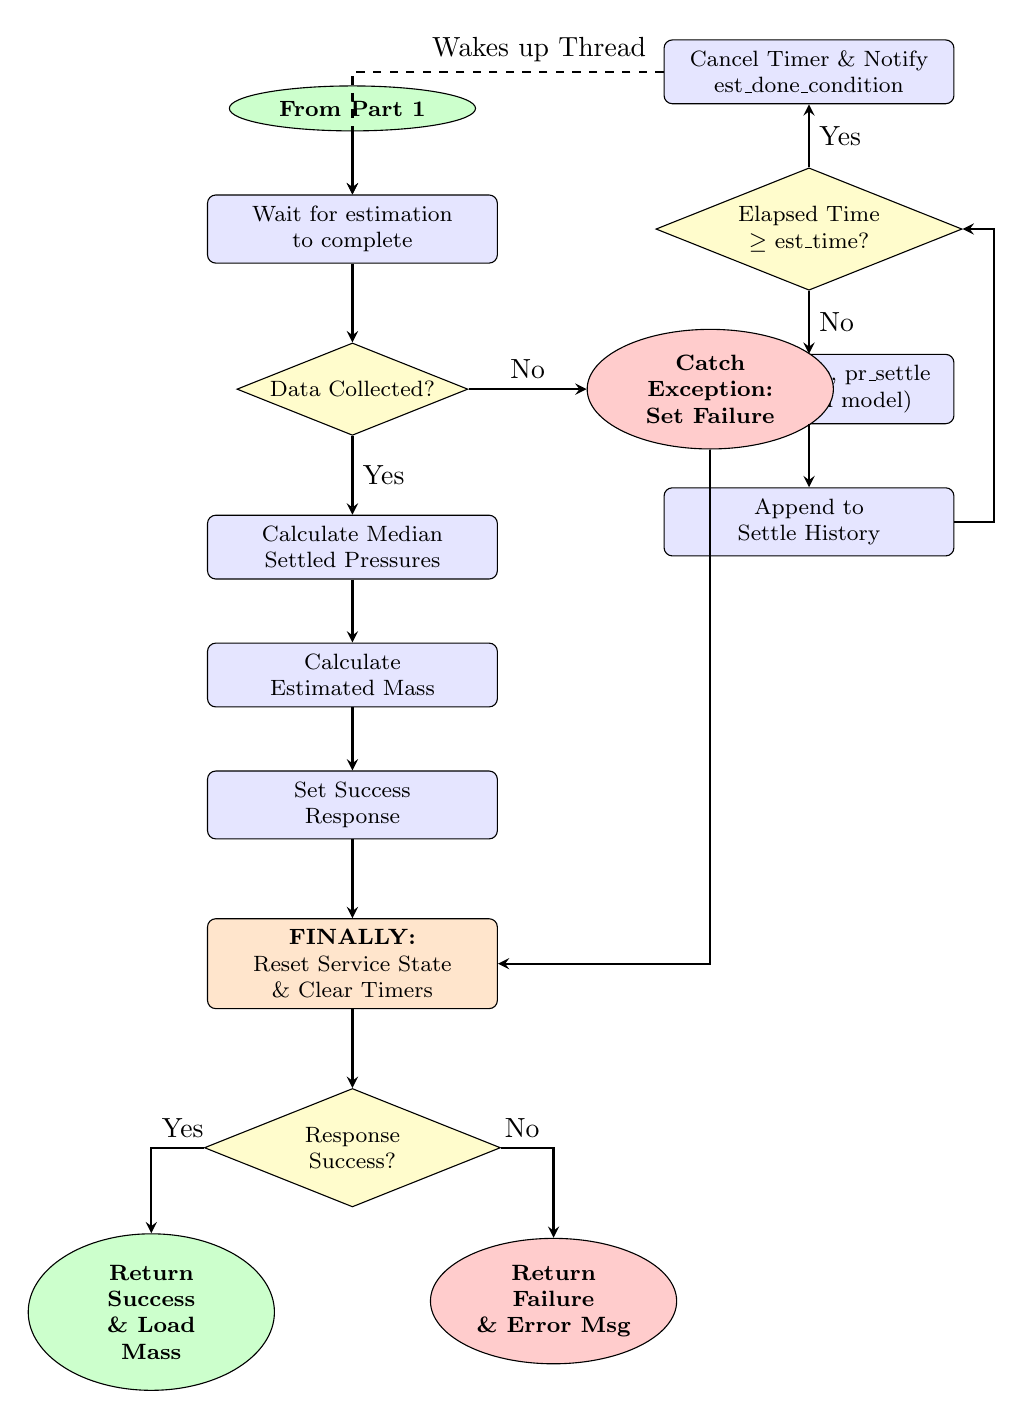
\begin{tikzpicture}[node distance=1.5cm, auto, >=latex']
    \tikzstyle{startend} = [draw, ellipse, fill=green!20, text width=2.0cm, text centered, font=\footnotesize\bfseries, inner sep=3pt]
    \tikzstyle{process}  = [draw, rectangle, fill=blue!10, text width=3.4cm, text centered, minimum height=0.7cm, rounded corners=3pt, font=\footnotesize, inner sep=4pt]
    \tikzstyle{decision} = [draw, diamond, fill=yellow!20, text width=2.2cm, text centered, aspect=2.5, font=\footnotesize, inner sep=1pt]
    \tikzstyle{success}  = [draw, ellipse, fill=red!20, text width=2.0cm, text centered, font=\footnotesize\bfseries, inner sep=3pt]
    \tikzstyle{arrow}    = [thick,->,>=stealth]

    \node [startend] (from1) {From Part 1};
    \node [process, below=0.8cm of from1] (wait) {Wait for estimation\\to complete};
    
    \node [decision, right=2cm of wait] (time) {Elapsed Time\\$\ge$ est\_time?};
    \node [process, below=0.8cm of time] (calc) {Calc pb\_settle, pr\_settle\\(exponential model)};
    \node [process, below=0.8cm of calc] (append) {Append to\\Settle History};
    \node [process, above=0.8cm of time] (cancel) {Cancel Timer \& Notify\\est\_done\_condition};

    \node [decision, below=1cm of wait] (collected) {Data Collected?};
    \node [success, right=1.5cm of collected] (catch) {Catch Exception:\\Set Failure};
    
    \node [process, below=1cm of collected] (median) {Calculate Median\\Settled Pressures};
    \node [process, below=0.8cm of median] (mass) {Calculate\\Estimated Mass};
    \node [process, below=0.8cm of mass] (successres) {Set Success\\Response};
    
    \node [process, fill=orange!20, below=1cm of successres] (finally) {\textbf{FINALLY:}\\Reset Service State\\\& Clear Timers};
    
    \node [decision, below=1cm of finally] (ret) {Response\\Success?};
    \node [startend, below left=1cm and 0.5cm of ret] (retsuccess) {Return Success\\\& Load Mass};
    \node [success, below right=1cm and 0.5cm of ret] (retfail) {Return Failure\\\& Error Msg};

    % Connections
    \draw [arrow] (from1) -- (wait);
    
    \draw [arrow] (time) -- node[right] {No} (calc);
    \draw [arrow] (calc) -- (append);
    \draw [arrow] (append.east) -- ++(0.5,0) |- (time.east);
    \draw [arrow] (time) -- node[right] {Yes} (cancel);
    \draw [arrow, dashed] (cancel) -| node[above, pos=0.2] {Wakes up Thread} (wait);

    \draw [arrow] (wait) -- (collected);
    \draw [arrow] (collected) -- node[above] {No} (catch);
    \draw [arrow] (collected) -- node[right] {Yes} (median);
    \draw [arrow] (median) -- (mass);
    \draw [arrow] (mass) -- (successres);
    \draw [arrow] (successres) -- (finally);
    \draw [arrow] (catch) |- (finally);
    
    \draw [arrow] (finally) -- (ret);
    \draw [arrow] (ret) -| node[above, pos=0.2] {Yes} (retsuccess);
    \draw [arrow] (ret) -| node[above, pos=0.2] {No} (retfail);

\end{tikzpicture}
}
\caption{Service Call: Data Collection \& Final Calculation}
\end{figure}

\subsection{Hardware Component}
\begin{itemize}
    \item \textbf{PT5400 Electronic Pressure Sensor} (installed at lift cylinder). 
\end{itemize}

% ==================================================================
% Section 4: Calibration Procedure
% ==================================================================
\section{Calibration Procedure}
\begin{quote}
\textit{Note: This procedure must be executed if another wheel loader model is used.}
\end{quote}

\subsection{Pressure Offset Model}
\begin{table}[H]
    \centering
    \caption{Empty Bucket Pressure Data for Offset Calibration}
    \begin{tabular}{c|c|c}
        \hline
        $\theta_g$ \textbf{(rad)} & $\mathbf{p_{bf}}$ \textbf{(ADC)} & $\mathbf{p_{rf}}$ \textbf{(ADC)} \\
        \hline
        0.1 & & \\
        0.2 & & \\
        0.3 & & \\
        0.4 & & \\
        0.5 & & \\
        0.6 & & \\
        0.7 & & \\
        \hline
    \end{tabular}
\end{table}

Fill the data in Table 1 while there is no load in the bucket. Use \texttt{linear} regression to find $p_{rf}(\theta_g)$, and treat $p_{rf}$ as a constant (average value), where $p_{rf}$ is the predicted pressure sensor value in ADC.

\subsection{Surface Fit Compensation Model}
\begin{table}[H]
    \centering
    \caption{Surface Fit Compensate Calibration Data}
    \begin{tabular}{c|c|c|c}
        \hline
        $\theta_g$ \textbf{(rad)} & \textbf{3\% Load} & \textbf{50\% Load} & \textbf{100\% Load} \\
        \hline
        0.1 & & & \\
        0.2 & & & \\
        0.3 & & & \\
        0.4 & & & \\
        0.5 & & & \\
        0.6 & & & \\
        0.7 & & & \\
        \hline
    \end{tabular}
\end{table}

Fill the load values (derived from the Simple Beam Model) in Table 2, and utilize the \texttt{sklearn} library to find the regression function $load_{est}(w, \theta_g)$, where $load_{est}$ is the final estimated load in tons.

% ==================================================================
% Section 5: Results and Analysis
% ==================================================================
\section{Results and Analysis}

\begin{quote}
\textit{Note: These results utilize regression constants derived from 0.1, 1.66, and 3.22 tons calibration loads (using water in the bucket).}
\end{quote}

By varying the load (water) and boom angle, the following metrics were calculated:
\begin{itemize}
    \item \textbf{RMSE\_s}: Load root mean square error due to $\theta_g$, indicating error affected by the boom angle.
    \item \textbf{RMSE\_w}: Load root mean square error due to the payload, indicating error affected by the actual load in the bucket.
\end{itemize}

\begin{figure}[h!]
    \centering
    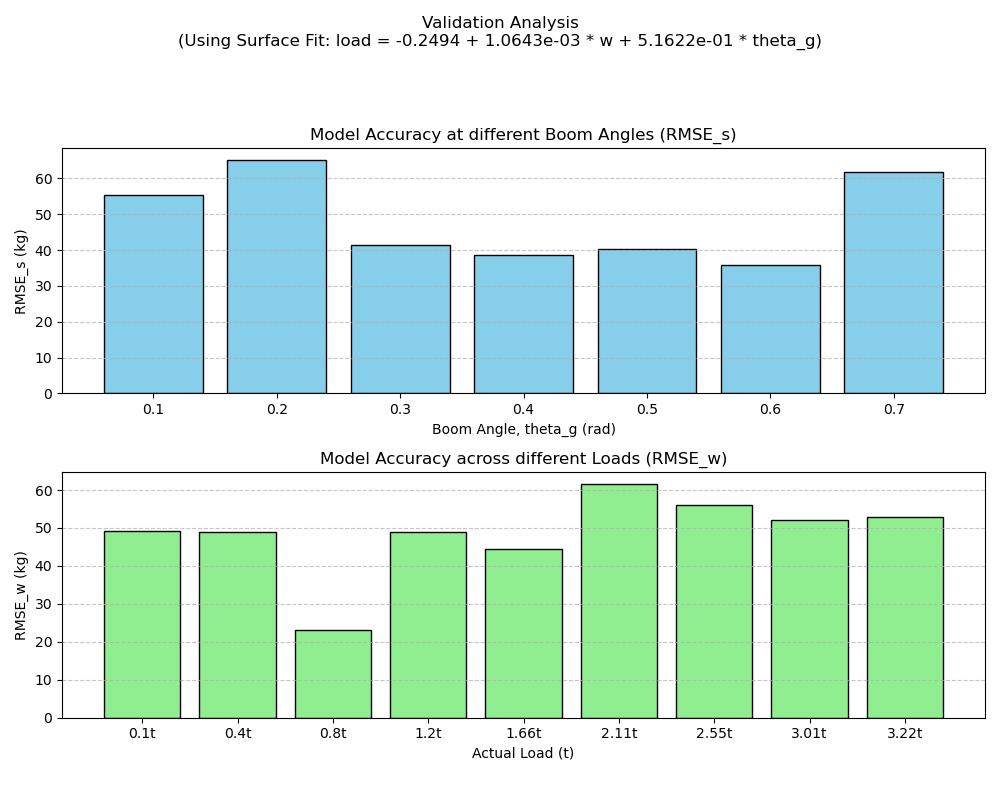
\includegraphics[width=0.9\textwidth]{../validation.png}
    \caption{Validation Analysis across different boom angles and actual payloads.}
\end{figure}

The implemented methodology yields a load estimation with an accuracy of \textbf{$\sim\pm 100\text{ kg}$} for a full bucket capacity of 3 tons, under the specified operating conditions ($\theta_g = 0.3 - 0.6\text{ rad}$).

% ==================================================================
% Section 6: Conclusion
% ==================================================================
\section{Conclusion}
This project successfully developed and validated a Hydraulic-Pressure Based Load Estimator for the XCMG958 autonomous wheel loader. By fusing data from a lift cylinder pressure sensor with a boom-chassis pin rotary encoder, filtering raw signals using Exponential Moving Average (EMA) models, and processing the inputs through a physical Simple Beam Model coupled with a data-driven Surface Fit Compensation regression, the system delivers precise payload feedback. 

Validated under static conditions on flat ground with the bucket at maximum tilt across a boom angle range of $\theta_g = 0.3 \text{ to } 0.6\text{ rad}$, the estimator achieves an exceptional accuracy of $\sim\pm 100\text{ kg}$ for a full bucket, easily satisfying the required $\pm 5\%$ ($\pm 160\text{ kg}$) accuracy threshold of the 3.2-ton full capacity. 

Furthermore, by utilizing a first-order pressure prediction model that estimates settled hydraulic pressures using only 1.0 second of static data, the system bypasses the physical 60-second stabilization delay to complete the entire process well within the target 3-second operational window. This high-speed performance effectively prevents inefficient ``run dry'' transport cycles by enabling instant payload verification and re-scooping commands, while simultaneously providing the loader's central controller with the real-time physical feedback required for adaptive kinematic control to optimize velocity, acceleration, and driving safety.

\end{document}